\section{Comments to the Group Work Experience}

\subsection*{Preferred working hours and days}

The bulk of the work was performed during the daytime. The spike at 9 am is a singularity, where one group member manually pushed 185 files because of an misunderstanding about git. Therefore, we conclude that the relevant productivity maximum was around 13 am. Afterwards, due to lunch time, the productivity decayed. Some pushes, where even performed during the night, which indicates the high commitment of the team.
\begin{figure}[h!]
\centering
\subfloat[daytime]{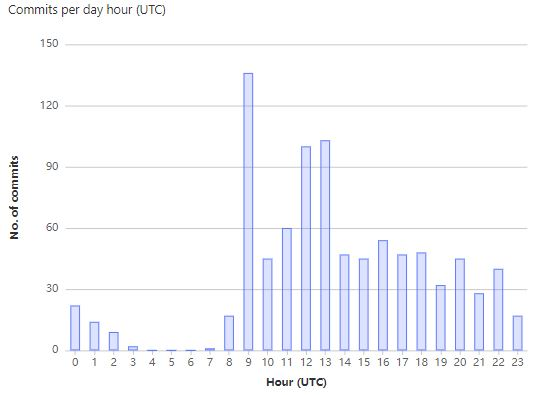
\includegraphics[width=0.5\linewidth]{group_work/hour_commits}}
\subfloat[monthday]{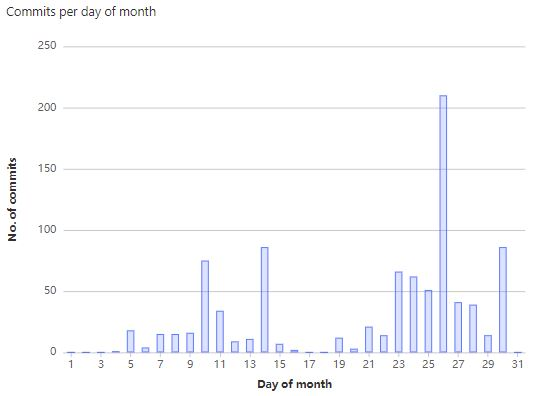
\includegraphics[width=0.5\linewidth]{group_work/monthday_commits}}\\
\subfloat[weekday]{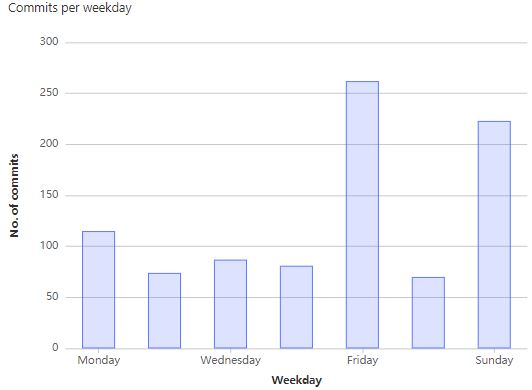
\includegraphics[width=0.5\linewidth]{group_work/weekday_commits}}
\caption{Commit histogram for different timescales.}
\label{fig:hour_commits}
\end{figure}
When we focus on a monthly scope, we can see spikes around the delivery dates at the end of the month and on the 14th for the third milestone. In a weekly scope, friday and sunday were the most populat days to push changes to the repository. This can be easily understood, when considering that the usual week of most team members was already packed with lectures, tutorials, and student jobs.

\begin{figure}[h!]
	\centering
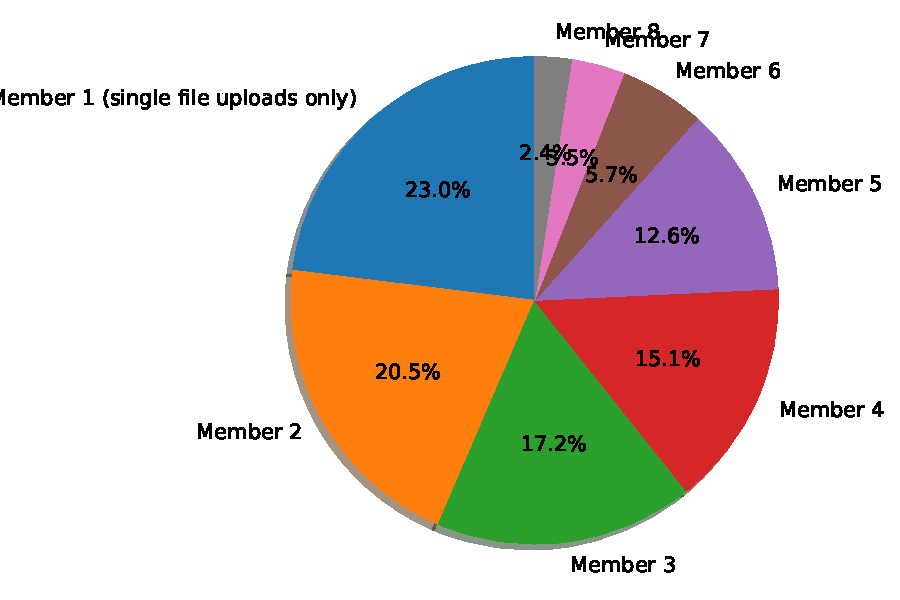
\includegraphics[width=0.7\linewidth]{group_work/name_commits}
\caption{Commits by group member.}
\end{figure}

\subsection*{Comparison to risk assessment}

Which risks where estimated wrongly?

\definecolor{lightgray}{rgb}{0.75,0.75,0.75}
\definecolor{lightergray}{rgb}{0.85,0.85,0.85}
\definecolor{slightlylightergray}{rgb}{0.92,0.92,0.92}
\def\checkmark{\tikz\fill[scale=0.4](0,.35) -- (.25,0) -- (1,.7) -- (.25,.15) -- cycle;}
\begin{center}
	\begin{footnotesize}
		\setlength{\arrayrulewidth}{1,05pt}
		\begin{tabular}[htb]{|p{2cm}|p{5cm}|p{1.5cm}|p{1cm}|p{1cm}|}
			\hline
			\textbf{Technical Risk} & \textbf{Countermeasures (CM)} &
			\textbf{Estimated prob.[\%]} &\textbf{CM needed} & \textbf{Threat avoided} \\
			\hline
			\hline
			\rowcolor{lightgray} Lack of access to data & Talk to the institution that possesses the data or ask the supervisors for access & 60.0 & \cmark & \cmark\\
			\hline	
			\rowcolor{lightgray} Lack of data & Find enough reliable resources before deciding on the final research question, & 50.0& \cmark & \cmark\\
			\hline
			\rowcolor{lightergray} Lack of knowledge & Read up things we need to learn in books or online & 40.0& \xmark & \cmark\\
			\hline
			\rowcolor{lightergray} Unreliable algorithm & Put more effort in the programming part, & 40.0&  \cmark& \cmark\\
			\rowcolor{lightergray} & Have enough team members with coding experience & &\xmark &\cmark\\
			
			\rowcolor{lightergray} & Check the references of research papers to find more data & &\cmark &\cmark\\
			\hline
			\rowcolor{lightergray} Personal biases (e.g. when categorizing data) & Try to find very objective ways to categorize data, although one can probably never be sure that this kind of bias does not occur & 40.0&\xmark & \cmark\\
			\hline	
			\rowcolor{lightergray} Bad or useless technology &  Find appropriate methods to create good model & 40.0 &\xmark & \cmark\\ 
			\hline
			\rowcolor{lightergray} Poorly formulated research question & If necessary, talk with the supervisors of the lecture whether (minor) changes are OK & 30.0 & \xmark & \cmark\\
			\hline
			\rowcolor{slightlylightergray} Data bias & try to get reliable data or at least try to find aspects which could lead to a bias in your data & 20.0& \cmark &\cmark\\
			\hline	
			\rowcolor{slightlylightergray} Insufficient idea of the project & Choose only a research question which is truly understood by the whole team & 20.0&\xmark &\cmark\\
			\hline
			\rowcolor{slightlylightergray} Irrelevant requirements & establish realistic requirements to complete the project & 10.0&\xmark &\cmark\\
			\hline	
			\rowcolor{slightlylightergray} Project too complex & With enough dedication and willpower, one can achieve everything & 10.0 &\xmark &\cmark\\
			\hline
		\end{tabular}
	\end{footnotesize}
\end{center}

\begin{center}
	\begin{footnotesize}
		\setlength{\arrayrulewidth}{1,05pt}
		\begin{tabular}[htb]{|p{2cm}|p{5cm}|p{1.5cm}|p{1cm}|p{1cm}|}
			\hline
			\textbf{Organizational Risk}& \textbf{Countermeasures (CM)} &
			\textbf{Estimated prob.[\%]} &\textbf{CM needed} & \textbf{Threat avoided} \\
			\hline
			\hline
			\rowcolor{lightgray} Poorly formulated priorities & Never formulate priorities by yourself, always work in a team! $\Rightarrow$ automatic cross-checks & 60.0&\xmark &\cmark\\
			\hline	
			\rowcolor{lightergray} Irrelevant resources & Check diligently if all resources are relevant & 40.0 &\xmark &\cmark\\
			\hline
			\rowcolor{slightlylightergray} Strong interdependence in the team & This might only be a problem in teams with poor communication and lazy students, which does not apply to our team & 10.0 &\cmark &\xmark\\
			\hline
		\end{tabular}
	\end{footnotesize}
\end{center}

\begin{center}
	\begin{footnotesize}
		\setlength{\arrayrulewidth}{1,05pt}
		\begin{tabular}[htb]{|p{2cm}|p{5cm}|p{1.5cm}|p{1cm}|p{1cm}|}
			\hline
			\textbf{Project Management Risk}& \textbf{Countermeasures (CM)} &
			\textbf{Estimated prob.[\%]} &\textbf{CM needed} & \textbf{Threat avoided} \\
			\hline
			\hline
			\rowcolor{lightgray} Wrong time estimation & This is a potentially dangerous risk, that is why time estimations have to be as precise as possible. We chose a democratic process where everybody assigns a workload he thinks is adequate to each task. The results are discussed afterwards and we decide on a time estimate together & 70.0&\xmark &\cmark\\
			\hline
			\rowcolor{lightergray} No control points & Try to set up synchronizing meetings to figure out problems with understanding or mistakes & 40.0  &\cmark &\cmark\\
			\hline
			\rowcolor{lightergray} Wrong task assignment & This is critical as well, which is why we try to let everybody assign himself to the tasks he feels comfortable with to ensure proper task assignment & 30.0 &\cmark &\cmark\\
			\hline	
			\rowcolor{lightergray} Bad team communication & Conduct weekly meetings as a minimum to synchronize the team, have more meetings if necessary & 25.0&\cmark &\cmark\\
		
			\hline
		\end{tabular}
	\end{footnotesize}
\end{center}

\begin{center}
	\begin{footnotesize}
		\setlength{\arrayrulewidth}{1,05pt}
		\begin{tabular}[htb]{|p{2cm}|p{5cm}|p{1.5cm}|p{1cm}|p{1cm}|}
			\hline
			\textbf{External Risk}& \textbf{Countermeasures (CM)} &
			\textbf{Estimated prob.[\%]} &\textbf{CM needed} & \textbf{Threat avoided} \\
			\hline
			\hline
			\rowcolor{slightlylightergray} Low working morale & Have weekly meetings as a minimum to synchronize the team, & 20.0&\cmark &\cmark\\
			\rowcolor{slightlylightergray} & have a group leader ("product owner" Philipp in our case), which is able to motivate the team & &\cmark &(\cmark)\\
			\hline
			\rowcolor{slightlylightergray} Computer crash/software error & Save all data in the cloud and have backups, & 15.0&\xmark &\cmark\\
			\rowcolor{slightlylightergray} & ask the university for rental laptops if a computer stops working completely & &\xmark &\cmark\\
			\hline	
			\rowcolor{slightlylightergray} Changes by supervisors of the lecture & We estimate the probability of this to happen as very low but we are sure that we could talk to the supervisors if problems arise from such changes & 5.0&\xmark &\cmark\\
			\hline
		\end{tabular}
	\end{footnotesize}
\end{center}
	%todo: spell check
	In summary, all technical risks could be avoided. The most important countermeasures where taken against the lack of data: We continously searched for more datasets when we changed our approach. 
	
	
	
	Organizational risks posed a challenge in an unexpected threat. Sometimes, team members could only be motivated by very short deadlines, which impeded the report writing. 
	
	%todo: formulate nicer
	We as a team always came up with a solution to tackle the problem and managed to deliver every milestone on time and with a good quality. The team had exceptional communication and team skills and responsibly shifted tasks when team members had time limitations or a weak internet connection.
	
	\section*{Updated time schedule}
	
	After 16 weeks of team work including multiple project deadline extensions, we want to give an update of the initial time schedule we handed in together with the research proposal. At a first glance, the changes in the deadlines of the milestones can be observed. Also, one will notice that the buffers shrinked to mostly one day. Initially, we planned approximately one week buffer for each milestone. This can be interpreted as that the buffers were calculated completely right, since there was always at least one day buffer remaining in the end and we were able to finish the project milestones in time. Still, the buffers shrinked due to problems which occured as we were working on the milestones. This behavior was to be expected and that is the reason why we included buffers. 
	
	Another major change was the front end task schedule. In contrast to the initial plan, we already started working on the front end in the second milestone in order to have an interactive visualization of the datasets we collected. This front end was kept up-to-date and extended during the rest of the project.
	
	Especially for milestone three, the task durations could be increased significantly due to the deadline extension until the 14th of August which was related to the exam period we went through. For all the other milestones, various minor changes in task durations and task schedules can be seen.
	
	The updated time schedule is shown in the following Figure \ref{fig:updated_time_schedule}.
	
	\begin{figure}[H]
		\centering
		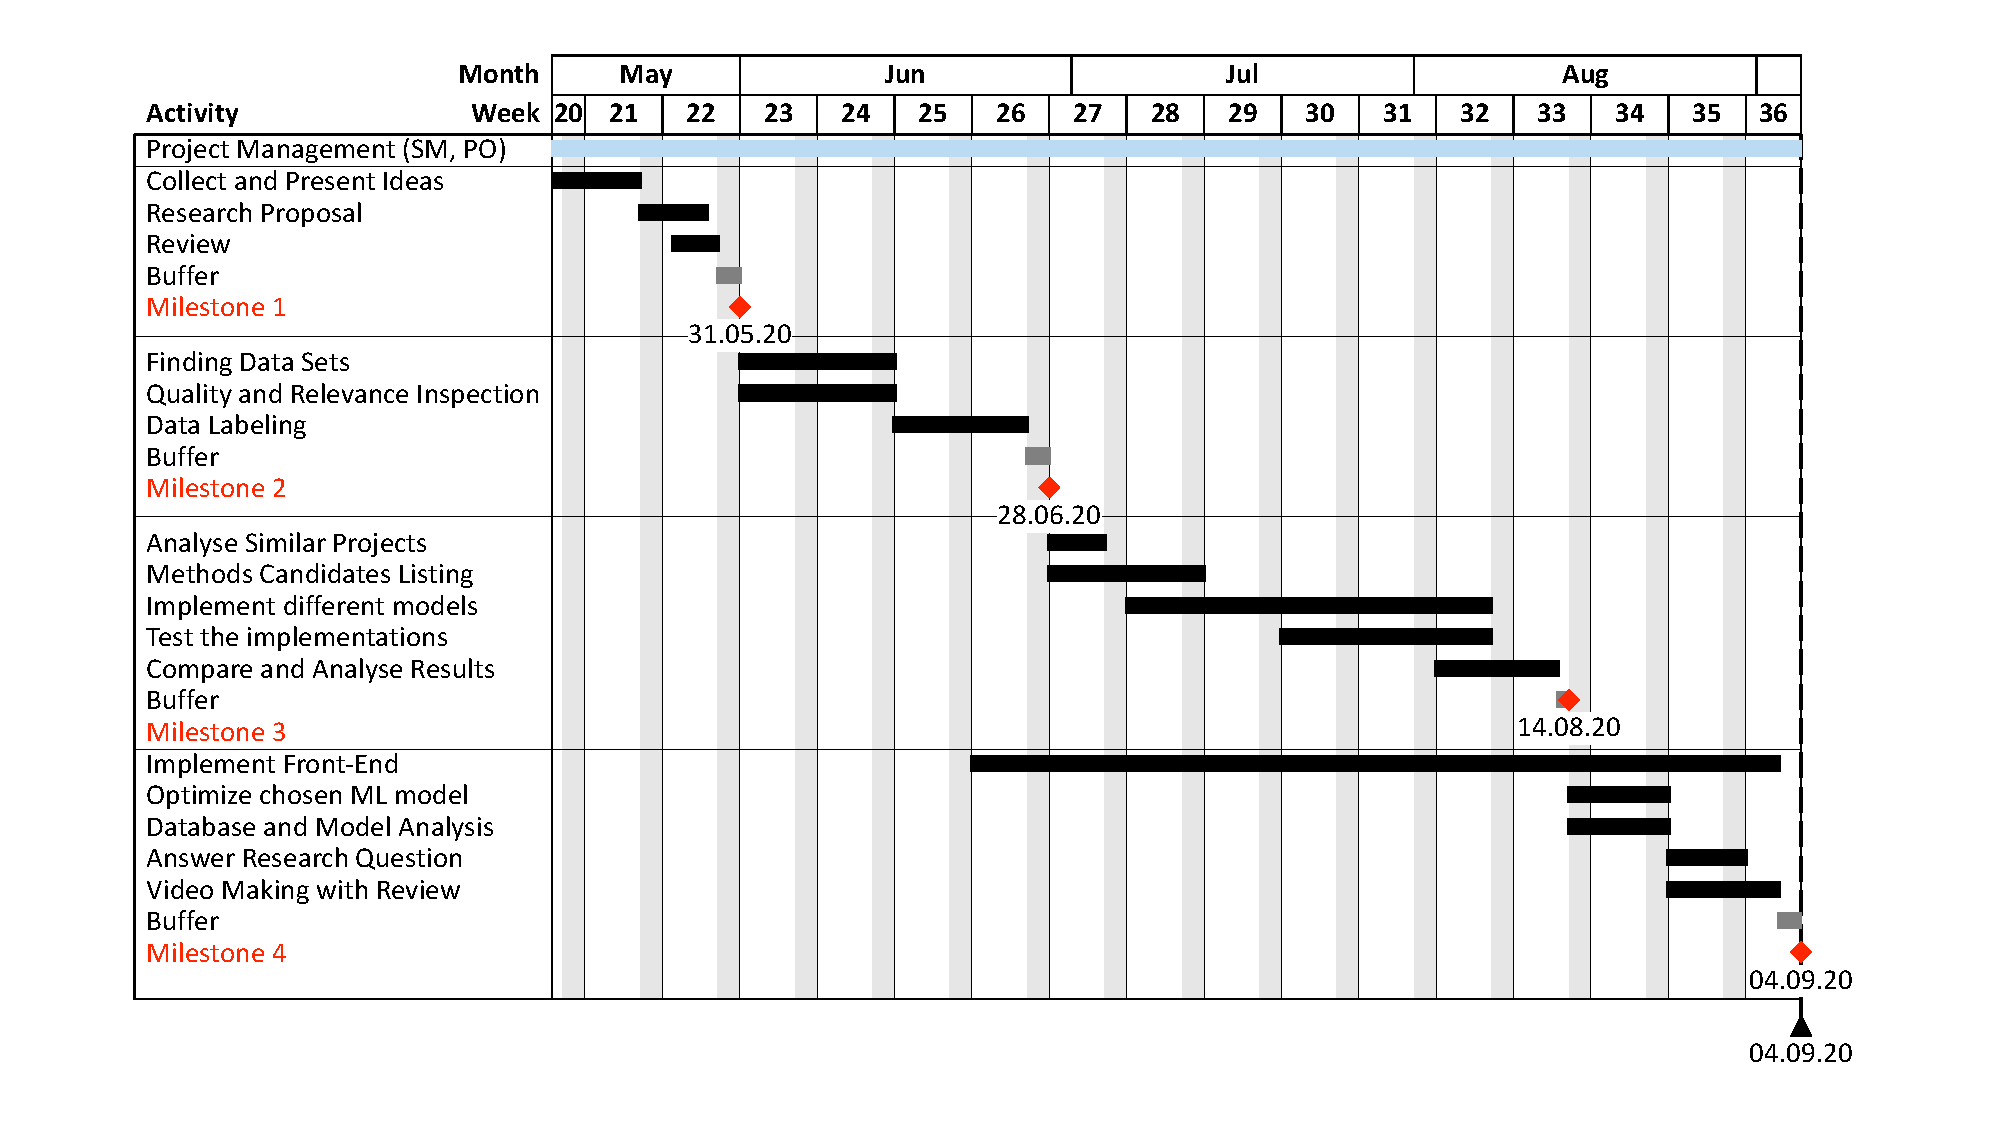
\includegraphics[width=\textwidth]{img/updated_time_schedule}
		\caption{Updated Time Schedule.}
		\label{fig:updated_time_schedule}
	\end{figure}
	
	
